\chapter{Dense coding in the prepare and measure scenario}
\label{chap:pam-quantum}

    Dense coding is an astonishingly straightforward use of quantum systems to improve the transmission of classical information. In sharp contrast to Holevo's bound \cite{holevo-bound-1973}, it allows for the lossless encoding of two dits in one single qudit. Entanglement between the communicating parties is the price to pay for that. In its original formulation \cite{bennett_1992_superdense}, dense coding is a device dependent protocol: Alice's encoding operators and Bob's measurements must be fully characterized. Already hinted in sec. \ref{sec:dense-coding} is the possibility of interpreting a type of prepare and measure scenario --- the one with quantum preparations, entanglement assistance, and a single measurement --- as a physical implementation of dense coding. In return, the characterization requirements are eased, and, remarkably, interesting properties can be inferred from imposing bounds on the amount of communication and observing the behaviors. Our task in this chapter is to define this device-independent formulation of dense coding and derive some first results. Among them, we will show how to build entanglement witnesses, self-test maximally entangled states, and optimize the preparations and measurements to better perform the protocol. Stepping in the direction of more general entanglement-assisted prepare and measure scenarios, we also provide a witness in the case where more measurements are allowed.

    These results were published in \cite{moreno_pamdense_2021}, and all their proofs are provided in appendix \ref{ap:pam-quantum}.


    %%%%%%%%%%%%%%%%%%%%%%%%%%%%%%%%%%%%%%%%%%%%%%%
    \section{Semi-device-independent dense coding}
    \label{sec:sdi-dense-coding}
        In dense coding, two parties share an entangled pair and communicate via a quantum state. Quantum communication happens one-way, and the transmitted state is of the same local dimension (w.r.t. the encoding device) as the entangled pair. The task is to encode a classical message $x \in \mathcal{X} \equiv \posrange{N-1}$, and it is known that two \emph{d}its ($N = d^2$) can be perfectly recovered from one qudit of communication, for some choices of a measurement with $N$ outcomes \cite{barenco_dense_1995}.
    
        Translating to the prepare and measure lingo, we let Alice and Bob share an entangled state $\rho \in \densop{\hilb_A \otimes \hilb_B}$ as a resource. Their local dimensions, $\dim{\hilb_A} = d_A$ and $\dim{\hilb_B} = d_B$, need not be the same, but Alice's preparation must be of dimension $d_A$. To achieve quantum advantage in the dense coding task, Alice and Bob must be able to exploit the correlations available in their entangled pair. Under the circumstances, her most general strategy is to apply a local transformation $\Lambda_x : \densop{\hilb_A} \mapsto \densop{\hilb_A}$ directly on her share of $\rho$, then send it to Bob. After that,
        %
        $$
            \rho \mapsto \left( \Lambda_x \otimes \id \right)\rho \equiv \rho_x
        $$
        %
        will be in his possession. It is crucial to enforce that
        %
        $$
            \ptr{A}{\rho_x} = \ptr{A}{\rho_{x^\prime}} \quad\forall x, x^\prime ,
        $$
        %
        a condition remindful of no-signaling, for it subsumes the fact the Alice's operations, being local, cannot affect Bob's marginal state. On his end, a good selection of a quantum measurement $\mathcal{M} = \{ E_b \}_{b=0}^{k-1}$ may provide advantage (over classical encodings) in the task of recovering her choice of $x$. Naturally, $\sum_b E_b = \id$, and each $E_b$ is a positive semidefinite operator acting on $\hilb_A \otimes \hilb_B$, which means to say he measures on both his and her transformed share of $\rho$. Summing it up, dense coding behaves in $\mathcal{Q}^\rho_{d_A,d_A^2,d_A^2,1}$, but we will also discuss some further generalizations.
        
        Many rounds of this protocols allow Alice and Bob to collectively infer the behavior
        %
        $$
            \mathbf{p} = \{ \condprob{b}{x} \}_{b,x} = \{ \tr{\rho_x E_b } \}_{b,x} .
        $$
        %
        From the behavior, we can assess their performance in the protocol. To that end, we assume that her choices of $x$ are equiprobable in $\mathcal{X}$ and define the figure of merit as
        %
        \begin{equation}
            p_{\text{suc}} = \frac{1}{N} \sum_{x=0}^{N-1} \condprob{b=x}{x} .
            \label{eq:psuc-dense-coding}
        \end{equation}
        %
        This is the very same average success probability discussed under the random access coding protocols of sec. \ref{sec:racs}, except that we now deal with a single measurement on Bob's side. Differently from the usual dense coding formulation --- which requires knowledge on the exact preparations and measurements employed ---, computing $p_{\text{suc}}$ relies solely on observational data. It is thus a device-independent figure of merit, completing our device-independent formulation of the dense coding protocol.
        
    %%%%%%%%%%%%%%%%%%%%%%%%%%%%%%%%%%%%%%%%%%%%%%%%%%%%%%%%
    \section{Witnessing and self-testing entanglement}

        Understanding the relationships between some figure of merit and the underlying resources is a commonplace question in device-independent scenarios. Important ones for the prepare and measure formulation of dense coding are which bounds the amount of entanglement in $\rho$ or its local dimensions imply on $\psuc$, and whether violating them witness or even self-tests some property of $\rho$. 
    
        Brunner et al. \cite{brunner_dimension_2013} considered similar questions in the quantum state discrimination scenario. Similarly to ours, their scenario allowed for a single measurement, and their figure of merit was equivalent to $\psuc$. However, the devices were independent, and their investigation focused on what could be inferred about quantum versus classical preparations. In chap. \ref{chap:pam}'s terminology, they were mostly interested in analyzing $\psuc$ in $\mathcal{C}_{d<N,N,N,1}$ against $\mathcal{Q}_{d<N,N,N,1}$. Interestingly, they found out both classical and quantum bounds for $\psuc$ are equal to $d_A / N$. Therefore, while that success probability can be used as a dimension witness, it cannot witness the type of preparations.
        
        Our first result generalizes theirs in the following way
        %
        \begin{restatable}[Schmidt number witness]{res}{schmidtnumber}
            Let $\rho$ be a shared resource with Schmidt number $s$ and local dimension $d_A$ on Alice's side. If she chooses one out of $N$ preparations, and Bob performs a single measurement with $N$ outcomes on the joint state, then
            %
            \begin{equation}
                \psuc \leq \min \left( \frac{d_A s}{N}, 1 \right) .
                \label{eq:result-1}
            \end{equation}
            %
            When $N \geq d_A s$, the bound is tight.
            \label{res:1}
            \label{res:schmidt-number-witness}
        \end{restatable}
        %
        Separable states ($s=1$) thus recover the bound $\psuc \leq d_A / N$ from \cite{brunner_dimension_2013}. For this reason, whenever the transmitted state's dimension is knowingly $d_A$, a $\psuc > d_A / N$ witness entanglement. Because only local operations are used to prepare the $\rho_x$, and those cannot increase $s$, any $\psuc > d_A s / N$ unambiguously certifies that $\rho \notin S_s$, so providing a lower bound on its Schmidt number.
        
        A particular instance of ineq. \ref{eq:result-1} can also be used for self-testing maximally entangled states.
        %
        \begin{restatable}[Self-testing maximally entangled states]{res}{selftest}
            In dense coding instances ($N=d_A^2$) of the prepare and measure scenario with $s=d_A$, saturation of ineq. \ref{eq:result-1} certifies, up to a local unitary transformation, that the shared state $\rho$ is maximally entangled.
            \label{res:self-testing-maximally-entangled}
        \end{restatable}
        
        Interestingly, this has implications for quantum key distribution protocols in the prepare and measure dense coding scenario. Suppose Alice does not actually share a maximally entangled pair with Bob, but rather with a third, malicious party that wants to eavesdrop on their communication. Let us suitably call her Eve. Apart from sharing a maximally entangled pair $\rho_{AE}$ with Alice, she intercepts Alice's communication of her share of $\rho_x$. From result \ref{res:self-testing-maximally-entangled}, she reads out $x$ with $\psuc = 1$, thus perfectly learning Alice's message. Because, at the end of the day, it will be Alice and Bob who share data to infer their $\psuc$, Eve must share a second maximally entangled pair $\rho_{EB}$ with Bob, which she exploits to reencode $x$ and transmit to Bob. In this way, Alice and Bob's $\psuc$ will saturate, tricking them into believing they share a maximally entangled pair. As Eve succeeds in eavesdropping without being detected, the prepare and measure dense coding protocol is not cryptographically secure.
        
        Historically, dense coding was introduced as a perfect encoding protocol. Relaxing this condition, by letting $\psuc < 1$, can shine more light on the role of entanglement assistance. Sharing pure entangled states, as the following result shows, is always advantageous over having only classical correlations (in the form of separable states).
        %
        \begin{restatable}[Pure states quantum advantage]{res}{purestates}
            Sharing a pure entangled state, which we write in the Schmidt decomposition $\ket{\psi} = \sum_{i = 0}^{s-1} \eta_i \ket{i} \otimes \ket{i}$, the best probability of success in the encoding of $N = d_A^2$ dits is lower bounded as
            %
            $$
                \psuc \geq \min \left( \frac{1 + \Gamma}{d_A}, \,1 \right),
            $$
            %
            where $\Gamma \equiv \sum_{i \neq j} \eta_i \eta_j \geq 0$.
        \label{res:pure-states-advantage}
        \end{restatable}
        
        From result \ref{res:1}, $N = d_A^2$ with $\rho \in \text{SEP}$ implies that $\psuc \leq 1 / d_A$, and as an entangled state is such that $\Gamma > 0$, all pure entangled states provide quantum advantage in the dense coding protocol.
        
        As a corollary, we have an amusing alternative proof to the possibility of perfectly encoding two dits in a qudit: a maximally entangled state has all $\eta_i = 1 / \sqrt{d_A}$ (c.f. sec. \ref{sec:states}), by which $\Gamma = d_A - 1$, thus $\psuc = 1$.
        
        Apropos of mixed states, a similar relation holds. Setting $d_A = d_B = d$ and making use of the singlet fraction $\zeta(\rho)$, which, in a loose sense, measures how much of a maximally entangled state is in $\rho$ (sec. \ref{sec:states}), it is true that
        %
        \begin{restatable}[Singlet fraction bound]{res}{singletfraction}
            The best probability of success achievable with a resource $\rho$ is lower bounded as
           \begin{equation}
                \psuc \geq \zeta(\rho) .
                \label{eq:psuc-singlet-fraction}
            \end{equation}
        \label{res:singlet-fraction-bound}
        \end{restatable}

        Interestingly, this fact closely links our witness to \emph{faithful entangled states}. These are defined to be those states whose entanglement can be certified by a fidelity-based witness, and it was recently proven that a state is faithful if and only if its singlet fraction is greater than $1/d$ \cite{guhne_faithful_2021}. Eq. \ref{eq:psuc-singlet-fraction} hence implies that any $\psuc > 1/d$ certifies $\rho$ is faithful. 
 
        As another application of this same result, consider an isotropic state (sec. \ref{sec:states})
        %
        $$
            \chi(\alpha) = \alpha \ketbra{\Phi^+}{\Phi^+} + (1 - \alpha) \frac{\id}{d^2} ,
        $$
        %
        which is separable only in the range $\alpha \leq \frac{1}{d + 1}$. Its singlet fraction is
        %
        $$
            \zeta\left[ \chi(\alpha) \right] = \alpha + \frac{1 - \alpha}{d^2} ,
        $$
        %
        and monotonically decreases with decreasing $\alpha$. As
        %
        $$
            \zeta \left[ \chi \left( \frac{1}{d + 1} \right) \right] = \frac{1}{d}
        $$
        %
        is the classical bound for $\psuc$ (result \ref{res:1}), it follows that $\psuc \geq \zeta(\rho)$ can witness entanglement for all isotropic states.        

        As pointed in sec. \ref{sec:states}, isotropic states are a common benchmark for quantum informational protocols. In particular, there are entanglement witnesses in the Bell nonlocality and quantum steering scenario that can certify a $\chi(\alpha)$ is entangled from some critical visibility $\alpha_{\text{crit}}$ upwards. Before contrasting them to our result, it is important to justify whether the comparison is fair. In the case of Bell nonlocality, it is not. Any prepare and measure scenario allows for communication, and all our witnesses rely on local dimension bounds, thus being only semi-device-independent. Contrastingly, Bell nonlocality is built on a causal structure with no direct relations between the parties, and is fully device-independent. Therefore, we expect any witness in this scenario to perform more poorly. The answer for quantum steering is not so clear-cut. While it also forbids communication, it does rely on local tomography for one of the parties. This presupposes full characterization of one measurement device, and hence also knowledge on the state dimension. Nevertheless, as made evident in fig. \ref{fig:isotropic-witness}, it does perform rather badly in comparison to our singlet fraction witness. The tests used were the Collins-Gisin-Linden-Massar-Popescu (CGLMP) inequality \cite{collins_cglmp_2002} and Wiseman et al.'s truncated harmonic series relation \cite{wiseman_2007_steering} (also stated in sec. \ref{sec:states}). CGLMP is not proven optimal for isotropic states, and in fact, for specific dimensions, better ones are known (e.g., \cite{divianszky_qutritwitness_2017}). On the other hand, the steering witness employed is only optimal for projective measurements. The case for POVMs is not so clear, and may lead to better witnesses \cite{nguyen_somemeasurements_2020}.
        
        \begin{figure}
            \centering
            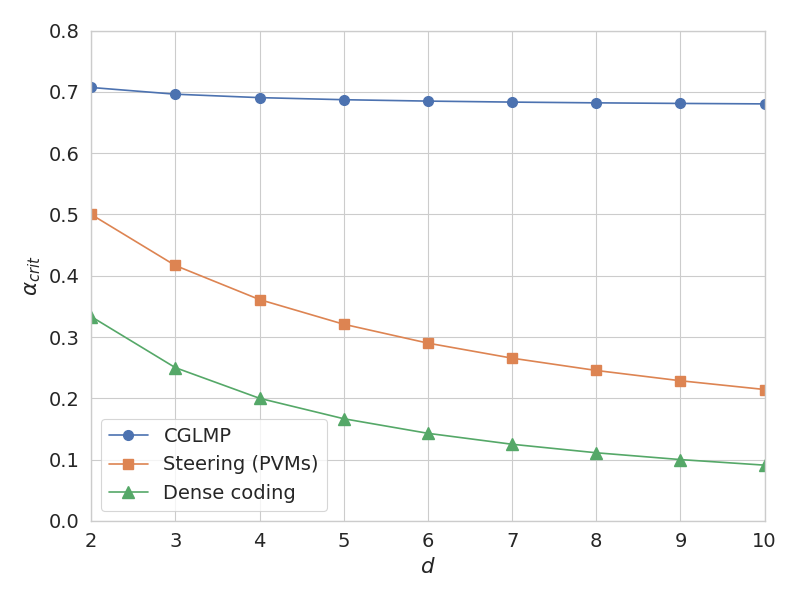
\includegraphics[width=.65\columnwidth]{isotropic-witness.png}
            \caption{Comparison between witness \ref{eq:psuc-singlet-fraction} to the CGLMP Bell inequality witness \cite{collins_cglmp_2002} and Wiseman et al.'s steering witness \cite{wiseman_2007_steering} for isotropic states (eq.~\eqref{eq:isotropic-states}). With a dimension assumption, the prepare and measure dense coding scenario can witness all entangled isotropic states. See the main text for a discussion on the fairness of this comparison.}
        \label{fig:isotropic-witness}
        \end{figure}
        
        Taking first step towards the study of more general entanglement assisted prepare and measure scenarios, we extend another result from the state discrimination task studied in \cite{brunner_dimension_2013}. In it, the authors allowed there to be $Y = N (N-1)/2$ dichotomic measurement choices, where $N$ is the number of preparations. Each measurement is labeled as the pair $(x, x^\prime)$, where $x > x^\prime$ with $x, x^\prime \in \posrange{N-1}$, and the behaviors now have elements $\condprob{b}{x,y}$. Their result states that, for uncorrelated parties, the expression
        %
        $$
            V_N \equiv \sum_{x > x^\prime} \abs{ \condprob{b=1}{x, (x, x^\prime)} - \condprob{b=1}{x^\prime, (x, x^\prime)} }^2 \leq \frac{N^2}{2} \left( 1 - \frac{1}{\min(d_A,N)} \right)
        $$
        %
        is a quantum dimension witness for any communication dimension $d_A < N$, and can also distinguish between quantum and classical systems (in the sense of pair-wise mutually commuting preparations, explained in sec. \ref{sec:quantum-behaviors}) for any $N$ which is not a multiple of $d$. By allowing for an entangled resource of Schmidt number $s$ between the parties, we found the following generalization.
        
        \begin{restatable}[Multiple measurements witness]{res}{moremeasurements}
            Given a shared bipartite resource with Schmidt number $s$, a prepare and measure scenario with $N$ $d_A$-dimensional preparations labeled by $x \in \posrange{N-1}$, and $N (N-1)/2$ dichotomic measurements labeled as $(x, x^\prime)$ for $x > x^\prime$ is such that
            %
            \begin{align*}
                V_N &\equiv \sum_{x > x^\prime} \abs{ \condprob{b=1}{x, (x, x^\prime)} - \condprob{b=1}{x^\prime, (x, x^\prime)} }^2 \\
                &\qquad\qquad\leq \frac{N^2}{2} \left( 1 - \frac{1}{\min(d_A s,N)} \right) .
            \end{align*}
            %
            If $s = d_A$, and $N < d_A^2$ or $N$ is an integer multiple of $d_A^2$, the inequality is tight.
            \label{res:more-measurements}
        \end{restatable}
        
        For fixed $N$ and $d_A$, $V_N$ can witness whether $\rho \in S_s$ or not.
    

    %%%%%%%%%%%%%%%%%%%%%%%%%%%%%%%%%%%%%%%%%%%%%%%%%%%%%%%%%%
    \section{Optimizing the dense coding probability of success}
    \label{sec:pam-quantum-optimization}

        Up until now, we have focused on what can be inferred about $\rho$ from the observable statistics. In practice, $\rho$ is sometimes treated as a resource to be consumed in the protocol, and it may be of interest to obtain the preparations $\rho_x$ and measurement $\mathcal{M} = \{ E_b \}$ that make the best use of it to achieve the largest $\psuc$. More formally, we are interested in solving
        %
        \begin{subequations}
            \begin{alignat}{2}
                &\text{given}    &\quad & \rho \\
                &\underset{\mathcal{M}, \Lambda_x}{\text{max.}}   &	  & \frac{1}{N} \sum_0^{N-1} \trb{ E_x \left( \Lambda_x \otimes \id \right) \rho} \label{eq:obj-func-cptp}\\
                &\text{s.t.}    &      & \Lambda_x \in \text{CPTP}, \quad\forall x \\
                &				   &	  & E_x \succeq 0, \quad\forall x \\
                &                  &      & \sum E_x = \id .
            \end{alignat}
            \label{eq:psuc-base-program}
        \end{subequations}
        %
        For an arbitrary $\rho$, this is a daunting task to approach analytically. Even numerically, the objective function is nonlinear, and optimizing over CPTP constraints is not directly a recognizable constraint. This lends little hope to the problem of efficiently finding global maxima. It is nevertheless possible to formulate an alternated semidefinite optimization procedure (also called \emph{see-saw} optimization) that solves to local extrema.

        Using channel-state duality (eqs.~\eqref{eq:channel-to-state} and \eqref{eq:state-to-channel}), the CPTP map $\Lambda_x$ can be cast as a bipartite state, for which the constraints of positivity and unit-trace are amenable to semidefinite programming. To see how, let $L_x \in \densop{\hilb_A \otimes \hilb_{A^\prime}}$ be the state dual to the channel $\Lambda_x : \densop{\hilb_A} \mapsto \densop{\hilb_{A^\prime}}$, where the superscript in $\hilb_{A^\prime}$ was added for ease of reading. Using $L_x$, the action of $\Lambda_x \otimes \id_B$ on the shared state $\rho$ is equivalent to $\ptrb{A}{(L_x \otimes \id_B) (\rho^{\intercal_A} \otimes \id_{A^\prime})} \in \densop{\hilb_{A^\prime} \otimes \hilb_B}$, where we only partially transpose $\rho$ because $\Lambda_x$ is local to Alice. Bob's measurement effects, $E_x$, will then act on $\densop{\hilb_{A^\prime} \otimes \hilb_{B}}$. Putting this into our objective function (eq.~\ref{eq:obj-func-cptp}), dropping the partial trace in favor of the trace, and completing $E_x$ to $\id_A \otimes E_x$ makes program~\eqref{eq:psuc-base-program} equivalent to
        %
        \begin{subequations}
            \begin{alignat}{2}
                &\text{given}    &\quad & \rho \\
                &\underset{\mathcal{M}, L_x}{\text{max.}}   &	  & \frac{1}{N} \sum_0^{N-1} \trb{ \left( L_x \otimes \id_B \right) \left(\rho^{\intercal_A} \otimes \id_{A^\prime} \right) \left( \id_A \otimes E_x \right)} \\
                &\text{s.t.}    &     & L_x \succeq 0, \quad\forall x \label{eq:constr-cp-map}\\
                &			    &	  & \ptr{A^\prime}{L_x} = \id_{A}, \quad\forall x \label{eq:constr-trace-preserving}\\
                &				&	  & E_x \succeq 0, \quad\forall x \\
                &               &     & \sum E_x = \id .
            \end{alignat}
            \label{eq:dense-coding-optimization}
        \end{subequations}
        %
        %where $^{\intercal_A}$ is a partial transposition on the $A$ system and the $L_x \in \mathcal{L} (\hilb_A \otimes \hilb_B)$ correspond to the preparations $\Lambda_x$. The constraints are all linear matrix inequalities (\ref{sec:sdp}), but the objective function is still nonlinear.
		These constraints are all linear matrix inequalities, and eqs.~\eqref{eq:constr-cp-map} and \eqref{eq:constr-trace-preserving} are in there to guarantee $L_x$ is completely positive and trace-preserving. We are closer to an SDP, but the objective function is still nonlinear. To circumvent that, we sample an initial measurement $\mathcal{M}^0$, fix it for the time being, and run program \ref{eq:dense-coding-optimization} only on the $L_x$ variables. The objective function is then clearly linear, and the last two constraints shall be removed. With the optimal (w.r.t. $\mathcal{M}_0$) $L_x$ from this first iteration, which we call $L_x^1$, fixed, optimizing over the measurements is also a semidefinite program. In this second step, the first two constraints may be left out, and we call its result $\mathcal{M}^1$. Together, $\mathcal{M}^1$ and $L_x^1$ are the result of the first iteration, and provide a lower bound on the best $\psuc$. After $N$ iterations, convergence can be tested through some heuristic criterion, such as checking whether $\psuc \left( \mathcal{M}^N, L_x^N \right) - \psuc \left( \mathcal{M}^{N-1}, L_x^{N-1} \right) \approx 0$. Different samples of $\mathcal{M}_0$ can lead to distinct results, and no formal guarantee of global extremality is provided by this procedure. Nonetheless, this is a computationally inexpensive procedure, thus running it for several initial samples and taking the best solution may provide numerical evidence of optimality. And, of course, one might as well start by sampling a $L_x^0$ and inverting the order of the programs.

        To see it in action, consider the Werner states (sec. \ref{sec:states}) parameterized as
        %
        \begin{equation}
            \rho_W ( \alpha ) = \frac{\id - \alpha S}{d^2 - \alpha d} ,
            \label{eq:werner-dense-coding}
        \end{equation}
        %
        where $d$ is the local dimension, $-1 \leq \alpha \leq 1$, and $S = \sum_{i,j=0}^{d-1} \ketbra{ij}{ji}$ is the swap operator. For $N = d^2$ preparations and a measurement with $N$ outcomes, we optimize the dense coding probability of success for $d \in \{2, \ldots, 5\}$ and a linear range over $\alpha$. Results are shown in fig. \ref{fig:werner-dense-coding-psuc}. All values of $\alpha \lesssim (d-1)/d$ saturate the classical (i.e., $s=1$) bound of $1/d$ from result \ref{res:1}, and every larger $\alpha$ violates it. In the inset, a comparison of $\psuc$ with the classical bound $1/d$, for $\alpha = 1$, suggests that Werner states of larger dimension provide smaller quantum advantages in dense coding.

		% \begin{figure*}[t!]
		% 	\newdimen\subfigcapmargin  \subfigcapmargin  =  -3em
		% 	\centering
		% 	%
		% 	\subfigure[]{\label{fig:werner-opt}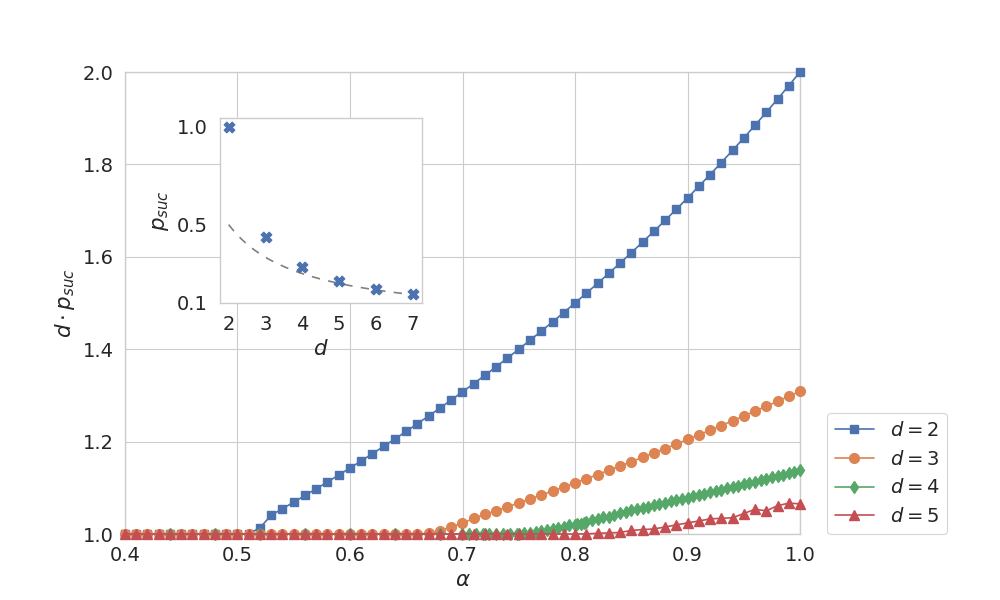
\includegraphics[width=.58\linewidth]{werner-opt.png}}\hfill
		% 	\subfigure[]{\label{fig:werner-opt-dims}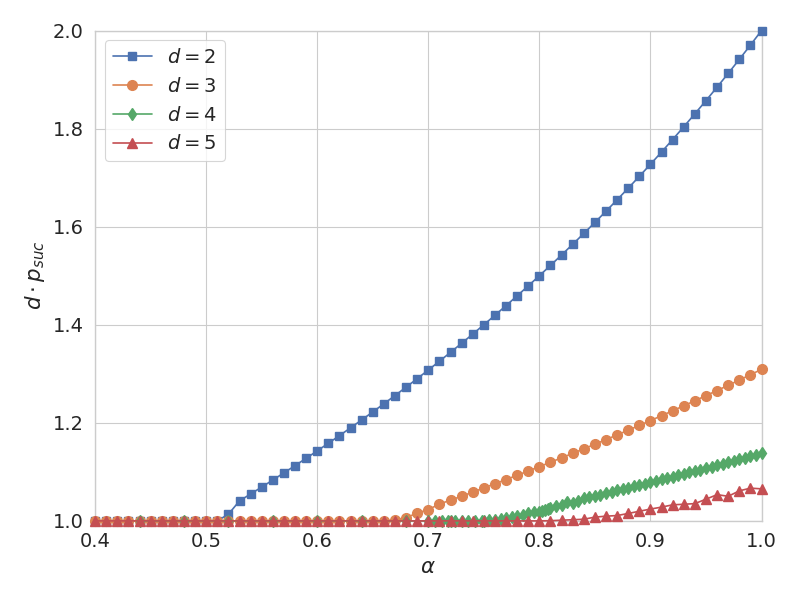
\includegraphics[width=.4\linewidth]{werner-opt-dims.png}}\hfill
		% 	%
        %     \caption{Optimal $\psuc$'s obtained for Werner states~\eqref{eq:werner-dense-coding} with the alternated optimization procedure over program~\eqref{eq:dense-coding-optimization}. Squares, circles, rhombuses and triangles correspond to $d = 2, 3, 4$ and $5$, respectively. Values are reescaled so that all classical bounds correspond to $1$. The inset shows $\psuc$ for $\alpha = 1$ (crosses) against the classical bound of $1/d$ in dimensions $2$ up to $7$.}
        % \label{fig:werner-dense-coding-psuc}
		% \end{figure*}
        
        \begin{figure}
            \centering
            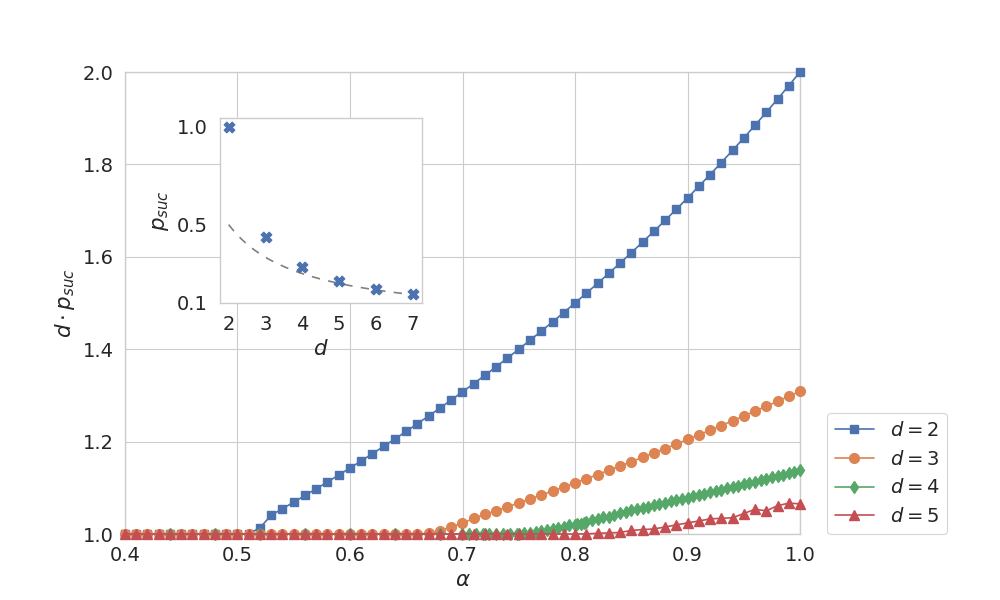
\includegraphics[width=.9\columnwidth]{werner-opt.png}
            \caption{Optimal $\psuc$'s obtained for Werner states~\eqref{eq:werner-dense-coding} with the alternated optimization procedure over program~\eqref{eq:dense-coding-optimization}. Squares, circles, rhombuses and triangles correspond to $d = 2, 3, 4$ and $5$, respectively. Values are reescaled so that all classical bounds correspond to $1$. The inset shows $\psuc$ for $\alpha = 1$ (crosses) against the classical bound of $1/d$ (dashed curve) in dimensions $2$ up to $7$.}
        \label{fig:werner-dense-coding-psuc}
        \end{figure}

    
    %%%%%%%%%%%%%%%%%%%%%%%%%%%%%%%%%%%%%%%%%%%%%%%%
    \section{Open questions}

    Regarding device-independent dense coding, an interesting possibility is to generalize its definition by allowing Alice's local dimension $d_A$ to be larger than the actual communicated qudit, i.e., to let $\Lambda_x : \densop{d_A} \mapsto \densop{d}$, with $d < d_A$. First discussions on that situation were recently started in \cite{nayak_rigidity_2020,tavakoli_eapam_2021}. As noted in \cite{tavakoli_eapam_2021}, in that case a road worth taking is to investigate if there are witnesses that do not depend on $d_A$, but only on the communicated state dimension. Application-wise, while the see-saw optimization procedure is reasonably efficient, it would be useful to better understand what types of guarantees regarding global optimality are possible to provide. Secondly, one could think of a conceptual explanation as to why higher dimensional Werner states are increasingly worse in outperforming the classical bound on $\psuc$, and whether this trend is also present in other classes of entangled states.

    General entanglement assisted prepare and measure scenarios --- and especially the one with quantum preparations --- are little explored in the literature. Most results hitherto presented are only valid for the $Y=1$ case, which is of special interest but begs for generalizations. Result \ref{res:more-measurements} is a small step in that direction. Simultaneously to our results, Tavakoli et al. provided important results on the same theme \cite{tavakoli_eapam_2021}, but much is still to be done.

    Below result \ref{res:self-testing-maximally-entangled}, we discussed how an eavesdropper could intercept Alice's communication while still tricking she and Bob into believing they share a maximally entangled resource. One interest in studying $Y > 1$ witnesses is that they may provide cryptographically secure tests. To see how, consider a BB84-like protocol \cite{bb84} where Alice, before sending her qubit, randomly chooses whether to apply a $\sigma_x$ gate to it. Up to an unmeasurable global phase, $\left( \ket{\Phi^+}, \ket{\Phi^-}, \ket{\Psi^+}, \ket{\Psi^-} \right) \overset{\sigma_x}{\longmapsto} ( \ket{\Psi^+}, \ket{\Psi^-}, \ket{\Phi^+}, \ket{\Phi^-})$. An eavesdropper sharing the entangled resource with Alice and measuring in the Bell basis would correctly get $x=0$ in the first situation, but wrongly guess $x=2$ in the latter. She could try switching to a $\sigma_x$-transformed Bell measurement, but without information on Alice's decision, this would be unhelpful. Worse than that, after mistaking $x$, she would send the wrong repreparation to Bob. During the whole protocol, Bob must also be blind to Alice's choice. Let us further suppose that he can choose between a standard Bell measurement or a $\sigma_x$-transformed one and that, to make ends meet, Alice sends $M + \delta$ qubits, where $M$ is the intended key size. Afterwards, Alice publicly announces the choices of $x$ and $\sigma_x$ she made on the extra $\delta$ messages. In all rounds when Bob made the correct decision on his measurements, his result should be perfectly correlated with Alice's encoding. If he observes some of them are not, he will know Eve eavesdropped. While this example is device dependent, it is of interest to find some witness for $Y=2$ that can device-independently guarantee security in a similar protocol, or prove there is none.